\documentclass[11pt,a4paper]{article}
\usepackage[utf8]{inputenc}
\usepackage[T1]{fontenc}
\usepackage{microtype}
\usepackage[margin=2cm]{geometry}
\usepackage{booktabs}
\usepackage{tabularx}
\usepackage{array}
\usepackage{enumitem}
\usepackage{xcolor}
\usepackage{tikz}
\usepackage{hyperref}
\usepackage{fancyhdr}
\usepackage{titlesec}
\usetikzlibrary{arrows.meta,positioning,calc,fit,backgrounds}

% Colors
\definecolor{c1color}{HTML}{1A5276}
\definecolor{c2color}{HTML}{7D3C98}
\definecolor{bothcolor}{HTML}{117A65}
\definecolor{lightgray}{HTML}{F2F2F2}
\definecolor{accent}{HTML}{D4AC0D}
\definecolor{setup}{HTML}{E8F0FE}
\definecolor{foundation}{HTML}{FFF3E0}
\definecolor{method}{HTML}{E8F5E9}
\definecolor{artifact}{HTML}{F3E5F5}
\definecolor{argument}{HTML}{E3F2FD}
\definecolor{closure}{HTML}{FBE9E7}
\definecolor{figcolor}{HTML}{5B2C6F}

% Hyperref
\hypersetup{colorlinks=true, linkcolor=c1color, urlcolor=c2color}

% Headers
\pagestyle{fancy}
\fancyhf{}
\rhead{\small\textit{Contribution Map}}
\lhead{\small\textit{From Creator to Orchestrator?}}
\rfoot{\thepage}
\renewcommand{\headrulewidth}{0.4pt}

% Section styling
\titleformat{\section}{\large\bfseries\color{c1color}}{}{0em}{}[\vspace{-0.3em}\rule{\textwidth}{0.8pt}]

% Tags
\newcommand{\ctag}[2]{\colorbox{#1}{\small\color{white}\textbf{#2}}}
\newcommand{\Cone}{\ctag{c1color}{C1}}
\newcommand{\Ctwo}{\ctag{c2color}{C2}}
\newcommand{\Cboth}{\ctag{bothcolor}{C1+C2}}
\newcommand{\figref}[1]{{\scriptsize\color{figcolor}\textbf{Fig\,#1}}}

\begin{document}

% ============================================================
% TITLE
% ============================================================
\begin{center}
{\LARGE\bfseries Contribution Map}\\[0.3em]
{\large From Creator to Orchestrator? --- Storyline at a Glance}\\[0.3em]
{\normalsize Internal document \quad|\quad \today}
\end{center}

\vspace{0.3em}

% ============================================================
% PAPER AT A GLANCE
% ============================================================
\begin{center}
\begin{tikzpicture}
\node[rounded corners=4pt, fill=lightgray, inner sep=6pt, text width=15.5cm, align=center] {
    {\small\textbf{$\sim$24 pages} \quad\textbullet\quad \textbf{3 figures} \quad\textbullet\quad \textbf{3 tables} \quad\textbullet\quad \textbf{53 references} \quad\textbullet\quad \textbf{8 sections + appendices}}\\[2pt]
    {\small Position paper \quad|\quad Design Science Research methodology \quad|\quad Reflexive demonstration}
};
\end{tikzpicture}
\end{center}

\vspace{0.3em}

% ============================================================
% THE TWO CONTRIBUTIONS
% ============================================================
\noindent
\begin{tabularx}{\textwidth}{@{} c X @{}}
\Cone & \textbf{Creator-to-Orchestrator Framework.} \textit{The position:} AI restructures knowledge work. The researcher shifts from producing text to directing, evaluating, and being accountable. If desk research is automatable, process alone is no longer a contribution. \\[0.3em]
\Ctwo & \textbf{Open Paper Machine.} \textit{The evidence:} An open-source LLM pipeline (Claude Opus 4.6 + MCP) that produced this manuscript. Serves as proof that the position is grounded in reality. \\
\end{tabularx}

\vspace{0.2em}
\begin{center}
\fcolorbox{accent}{white}{\parbox{0.72\textwidth}{\centering
\textbf{C2 is in service of C1.} The artifact is the evidence for the position.\\
The Open Paper Machine (C2) is the hammer. The nail is C1.}}
\end{center}

\vspace{0.5em}

% ============================================================
% STORYLINE ARC --- TikZ graphic
% ============================================================
\section{The Storyline}

\begin{center}
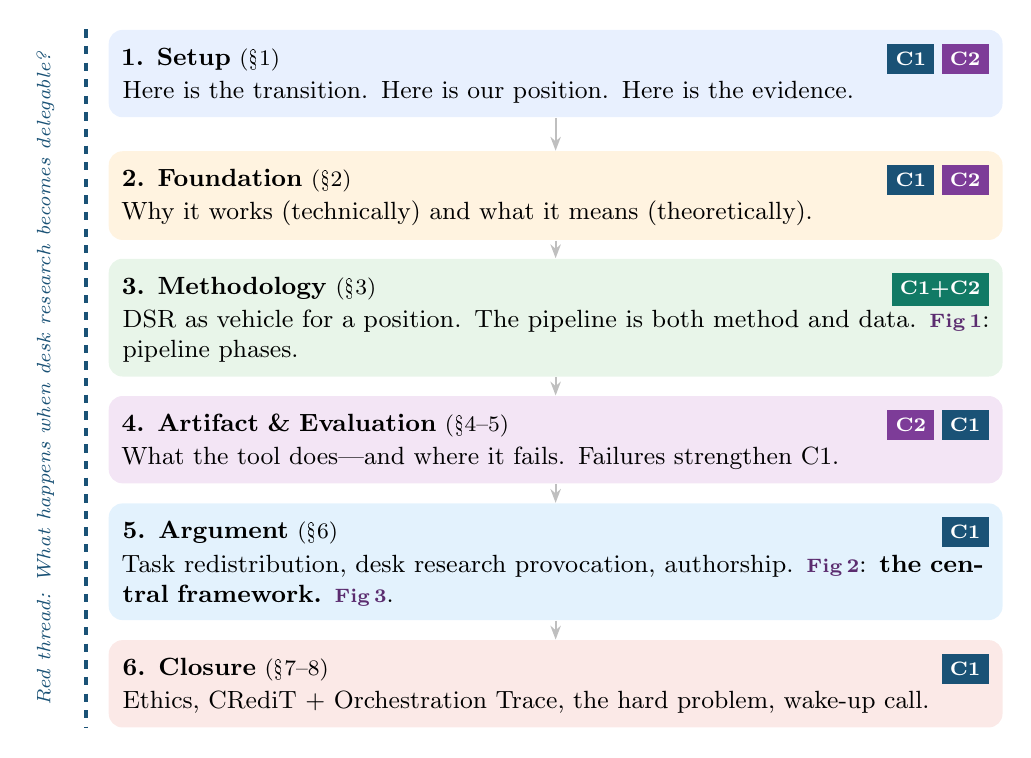
\begin{tikzpicture}[
    phase/.style={
        rounded corners=5pt,
        minimum height=1.05cm,
        text width=11cm,
        align=left,
        font=\small,
        inner sep=5pt
    },
    arrow/.style={-{Stealth[length=5pt]}, thick, gray!50},
    tag/.style={font=\scriptsize\bfseries, text=white, rounded corners=2pt, inner sep=2pt, minimum width=3em}
]

% Vertical phase boxes (top to bottom)
\node[phase, fill=setup] (p1) at (0,0)
    {\textbf{1. Setup} {\footnotesize(\S1)} \hfill \colorbox{c1color}{\color{white}\scriptsize\bfseries C1}\;\colorbox{c2color}{\color{white}\scriptsize\bfseries C2}\\[1pt]
     {\small Here is the transition. Here is our position. Here is the evidence.}};

\node[phase, fill=foundation] (p2) at (0,-1.55)
    {\textbf{2. Foundation} {\footnotesize(\S2)} \hfill \colorbox{c1color}{\color{white}\scriptsize\bfseries C1}\;\colorbox{c2color}{\color{white}\scriptsize\bfseries C2}\\[1pt]
     {\small Why it works (technically) and what it means (theoretically).}};

\node[phase, fill=method] (p3) at (0,-3.1)
    {\textbf{3. Methodology} {\footnotesize(\S3)} \hfill \colorbox{bothcolor}{\color{white}\scriptsize\bfseries C1+C2}\\[1pt]
     {\small DSR as vehicle for a position. The pipeline is both method and data. \figref{1}: pipeline phases.}};

\node[phase, fill=artifact] (p4) at (0,-4.65)
    {\textbf{4. Artifact \& Evaluation} {\footnotesize(\S4--5)} \hfill \colorbox{c2color}{\color{white}\scriptsize\bfseries C2}\;\colorbox{c1color}{\color{white}\scriptsize\bfseries C1}\\[1pt]
     {\small What the tool does---and where it fails. Failures strengthen C1.}};

\node[phase, fill=argument] (p5) at (0,-6.2)
    {\textbf{5. Argument} {\footnotesize(\S6)} \hfill \colorbox{c1color}{\color{white}\scriptsize\bfseries C1}\\[1pt]
     {\small Task redistribution, desk research provocation, authorship. \figref{2}: \textbf{the central framework.} \figref{3}.}};

\node[phase, fill=closure] (p6) at (0,-7.75)
    {\textbf{6. Closure} {\footnotesize(\S7--8)} \hfill \colorbox{c1color}{\color{white}\scriptsize\bfseries C1}\\[1pt]
     {\small Ethics, CRediT + Orchestration Trace, the hard problem, wake-up call.}};

% Arrows between phases
\draw[arrow] (p1.south) -- (p2.north);
\draw[arrow] (p2.south) -- (p3.north);
\draw[arrow] (p3.south) -- (p4.north);
\draw[arrow] (p4.south) -- (p5.north);
\draw[arrow] (p5.south) -- (p6.north);

% Red thread on the left
\draw[very thick, c1color, dashed] ([xshift=-8pt]p1.north west) -- ([xshift=-8pt]p6.south west);
\node[font=\scriptsize\itshape, text=c1color, rotate=90, anchor=south] at ([xshift=-16pt]$(p3.west)!0.5!(p4.west)$) {Red thread: What happens when desk research becomes delegable?};

\end{tikzpicture}
\end{center}

\vspace{0.3em}

% ============================================================
% SECTION MAP --- compact table
% ============================================================
\section{Section-by-Section}

\renewcommand{\arraystretch}{1.12}
{\small
\begin{tabularx}{\textwidth}{@{} l c X @{}}
\toprule
\textbf{Section} & \textbf{Tag} & \textbf{Function in Storyline} \\
\midrule
\S1.1 Intro & \Cone & Position declaration. Core question. Urgency. \\
\S1.2 RQs & \Cboth & RQ1 = what (tool), RQ2 = so what (argument) \\
\S1.3 Contributions & \Cboth & Intellectual contract: C1 primary, C2 as evidence \\
\midrule
\S2.1--2.3 Tech & \Ctwo & \textit{Why} the tool works: transformers, alignment, MCP \\
\S2.4--2.6 Theory & \Cone & \textit{What it means}: distributed cognition, sociotechnical, Autor \\
\S2.7--2.8 Risk & \Ctwo & Hallucination risk; landscape positioning (Table 1) \\
\midrule
\S3.1 DSR & \Cboth & DSR as vehicle for a position, not as validation \\
\S3.2 Pipeline & \Cboth & The artifact IS the data for the argument \hfill \figref{1} \\
\midrule
\S4 Tech Stack & \Ctwo & Components short. Design = pipeline, not parts \\
\S5.1--5.2 Cap./Fail. & \Cboth & Successes prove delegability; failures prove orchestrator need \\
\S5.3 Boundaries & \Cboth & Where human judgment is irreplaceable \\
\midrule
\S6 Opening & \Cone & The central framework --- Creator $\to$ Orchestrator \hfill \figref{2} \\
\S6.1 Task Redistr. & \Cone & Autor applied: delegated / retained / emergent tasks \\
\S6.2 Desk Research & \Cone & \textbf{Sharpest argument}: automatable $\rightarrow$ not a contribution \\
\S6.3 Augmentation & \Cone & \textit{How} the human engages (Davenport \& Kirby) \\
\S6.4 Authorship & \Cone & Accountability-based framework \hfill \figref{3} \\
\S6.5 Peer Review & \Cboth & New review mechanisms needed \\
\S6.6 Evolving Role & \Cone & Three dimensions: judgment, expertise, institutions \\
\midrule
\S7 Ethics & \Cboth & Authorship, integrity, bias --- honest and short \\
\S8.1--8.2 Conclusion & \Cboth & CRediT + Orchestration Trace = practical instruments \\
\S8.3--8.4 Hard Problem & \Cone & ``The technology is ready. The institutions are not.'' \\
\bottomrule
\end{tabularx}
}

\vspace{0.6em}

% ============================================================
% FIGURE MAP
% ============================================================
\noindent\textbf{\color{c1color}Figure Map}
\vspace{0.2em}

\renewcommand{\arraystretch}{1.1}
{\small
\begin{tabularx}{\textwidth}{@{} l l c X @{}}
\toprule
\textbf{Fig} & \textbf{Location} & \textbf{Tag} & \textbf{What it shows} \\
\midrule
1 & \S3.2 & \Cboth & Six-phase pipeline with human quality gates \\
\rowcolor{argument!50}
\textbf{2} & \textbf{\S6} & \Cone & \textbf{Creator-to-Orchestrator shift --- THE central figure} \\
3 & \S6.4 & \Cone & Accountability-based authorship (Asatiani 2021) \\
\bottomrule
\end{tabularx}
}

\vspace{0.6em}

% ============================================================
% BALANCE BAR
% ============================================================
\begin{center}
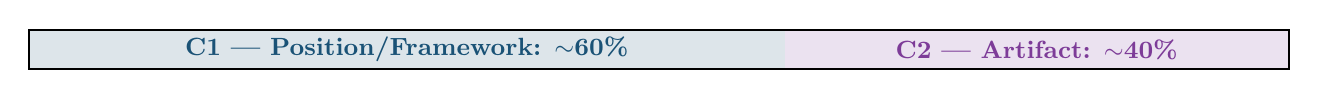
\begin{tikzpicture}
\fill[c1color!15] (0,0) rectangle (9.6,0.5);
\fill[c2color!15] (9.6,0) rectangle (16,0.5);
\node[font=\small\bfseries, text=c1color] at (4.8,0.25) {C1 --- Position/Framework: $\sim$60\%};
\node[font=\small\bfseries, text=c2color] at (12.8,0.25) {C2 --- Artifact: $\sim$40\%};
\draw[thick] (0,0) rectangle (16,0.5);
\end{tikzpicture}
\end{center}

\noindent{\small\textit{Verdict:} C2 always framed as evidence for C1. This is the correct balance for a position paper.}

\end{document}
